% !TEX root = ../main_lecture_notes.tex
\chapter{Table de mortalité}\label{chap:mortality_table}

En assurance-vie, les modèles de projections des cash-flows permettant d'évaluer les engagement de l'assureur repose sur l'utilisation de tables de mortalités. Il s'agit d'un tableau comprenant pour chaque âge $x$ la probabilité de décès avant d'atteindre l'âge $x+1$. Les probabilités de décès peuvent variées en fonction du genre des individus. la réglementation (Article A132-1 à A132-19 du codes des assurance\footnote{\url{https://www.legifrance.gouv.fr/codes/article_lc/LEGIARTI000035514715}}) impose l'utilisation de tables réglementaires TH et TF $00-02$ pour l'évaluation des engagements liées aux garanties décès. Les tables de mortalités peuvent inclure 
\begin{itemize}
\item l'année calendaire pour prendre en compte une situation particulière lié à une année (par exemple une pandémie mondiale)
\item l'année de naissance des individus (génération ou cohortes) pour capter l'allongement progressif de la durée de vie des individus. 
\end{itemize}
L'évaluation des engagements pour les garanties viagère se fait en utilisant des tables réglementaires par génération TGH et TGF $05$ qui fournissent une table de mortalité pour chaque année de naissance. Les assureurs peuvent aussi utiliser une table de mortalité d'expérience s'ils considèrent que le risque de mortalité pour leur portefeuille d'assurés diffère significativement du risque pour la population générale. Les probabilités de décès, la méthode de calculs et les données utilisées doivent être audité par un actuaire indépendant certifié. Les méthodes vues dans ce chapitre sont présentées dans le cadre de la mortalité mais peuvent s'appliquer dans d'autre contexte pour construire des lois de rachat, d'entrée en incapacité, en invalidité ou en dépendance, des lois de maintien en incapacité.
\section{Estimation des probabilités de décès et des taux de mortalité}\label{sec:mortality_rate}
\subsection{Notations et donées}\label{sssec:notation}
Soit $T$ la durée de vie d'un individu. Supposons que l'on dispose d'information sur un nombre $N$ d'individus
\begin{itemize}
  \item $\Data = \{t_i\}$: âge exacte de décès
  \item $\Data =\{x_i, \delta_i\}$: âge exacte de décès censuré
  \item $\Data = \{E^0_x,d_x\}$: nombre de survivant et nombre de décès à l'âge $x$
\end{itemize}
Nous pouvons estimer la fonction de survie $\widehat{S}(t)$. Dans l'étude de la mortalité on s'intéresse à la durée de vie résiduelle à l'âge $x$ défini par 
$$
T_x\sim T-x|T>x.
$$
On s'intéresse au quantités présentées dans le \cref{tab:incap_data}
\begin{table*}[ht!]\centering
% \ra{1.3}
\begin{tabular}{@{}lllll@{}}
\toprule
$E_x^0$&&&&Exposition initiale\\
&&&&Nombre de survivant jusqu'à l'âge $x$\\
\midrule
$E_x^c$&&&$(E_x^0 + E_{x+1}^0)/2 $&Exposition centrale\\

&&&$\sum_{i=1}^N\tau_{x,i}$&Cumul des temps d'observation d'individu d'age $x$\\
\midrule

$d_x$&&&$E^0_{x} - E^0_{x+1}$&Nombre de décès à l'âge $x$\\
\midrule
$q_x$&$\Prob(T_x \leq 1)$&$\Prob(T \leq x+1|T> x)$&$d_x/E^0_x$& Probabilité de décès d'un individu d'âge $x$ \\
&&&$1-\e^{-d_x/E_x^c}$&avant d'atteindre l'âge $x+1$\\
\midrule
$p_x$&$\Prob(T_x > 1)$&$\Prob(T > x+1|T> x)$&$1-q_x$ &Probabilité de survie d'un individu d'âge $x$ \\
&&&&jusqu'à l'âge $x+1$\\
\midrule
$\,_tp_x$&$\Prob(T_x > t)$&$\Prob(T > x+t|T> x)$&$\prod_{s=1}^tp_{x+s}$& Probabilité de survie d'un individu d'âge $x$ \\
&&&&jusqu'à l'âge $x+t$\\
\midrule
$\,_tq_x$&$\Prob(T_x \leq t)$&$\Prob(T \leq x+t|T> x)$&$1 - \,_tp_x$& Probabilité de décès d'un individu d'âge $x$ \\
&&&&avant d'atteindre l'âge $x+t$\\
\midrule

$\mu_x$&\multicolumn{2}{c}{$\lim_{h\rightarrow 0}h^{-1}\Prob(T_x\in[x,x+h])$}&$-\log(p_x)$ &Taux de décès instantanée à l'âge $x$\\
\midrule
$e_x$&$\E(T_x)$&$\E(T-x|T>x)$&$\sum_{t\geq 0} \,_tp_x$ &Espérance de vie résiduelle à l'âge $x$\\
\bottomrule
\end{tabular}
\caption{Récapitulatif des notations des tables de mortalités}
\label{tab:notation_mortality_table}
\end{table*}
Les estimateurs des quantités d'intérêts $q_x, p_x$ et $\mu_x$ utilisent les expositions et les nombre de décès $d_x$. Leur justification est donnée dans la section suivante.
\subsection{Estimation}
La justification de l'expression des estimateurs du \cref{tab:notation_mortality_table} repose sur la maximisatiuon de la vraisemblance des données. Les données de mortalités se limitent aux effectifs par âge $E^0_x$, avec $\Data = \{E^0_x\}_{x\in\mathbb{N}}$. Un extrait de la table réglementaire $TF 00-02$ est donné par \cref{tab:TF002}.
\begin{table}[ht!]
\centering
\begin{tabular}{ll}
  \hline
 Age & $l_x$ \\ 
  \hline
 $0$ & $100,000 $\\ 
 $1$ &$ 99,616 $\\ 
 $2$ &$ 99,583 $\\ 
 $3$ &$ 99,562 $\\ 
 $4$ &$ 99,545 $\\ 
 $\vdots$ &$\vdots $\\
 $111$ & $4$ \\ 
 $112$ & $1$ \\ 
   \hline
\end{tabular}
\caption{Extrait de la table de mortalité $TF 00-02$.}
\label{tab:TF002}
\end{table}
\begin{remark}
$l_x$ correspond à un nombre de survivant jusqu'à l'âge $x$. La taille initiale de la population (le radix) est noté $l_0$. Il s'agit d'une version normalisée des tailles de population observées telle que 
$$
l_x = \Prob(T>x)\cdot l_0
$$
\end{remark}

\subsubsection{Modèle binomial: estimation des $q_x$}\label{ssec:deces_binomial}
Le nombre décès $D_x$ à l'âge $x\in\mathbb{N}$ (Approche dite discrète) est une variable aléatoire binomial $D_x\sim \BinomialDist(E^0_x, q_x)$. L'application du maximum de vraisemblance conduit à 
$$
\widehat{q}_x = \frac{d_x}{E^0_x}.
$$
Pour $E^0_x\rightarrow \infty$, nous avons l'approximation suivante 
$$
\widehat{q}_x\sim\NormalDist\left(q_x, \frac{q_x(1-q_x)}{E^0_x}\right),
$$
qui permet de construire des intervalle de confiance.
\subsubsection{Modèle de Poisson: estimation des $\mu_x$}
Le temps de survie résiduelle $T_x$ à l'âge $x\in \RL_+$ (Approche dite continue) suit une loi exponentielle $\ExpDist(1/\mu_x)$. Cela implique que 
$$
q_x = 1-p_x = 1-\exp\left(-\int_{x}^{x+1}\mu_s\text{d}s\right).
$$
Il est usuel de supposer que $s\mapsto \mu_s$ constant entre deux âge $x$ et $x+1$, c'est à dire 
$$
\mu_s = \sum_{x\geq 0}\mu_x\ind_{[x,x+1)}(s).
$$
Ce modèle revient à supposer que le nombre de décès $D_x$ à l'âge $x$ suit une loi de Poisson $D_x\sim\PoissonDist(E_x^c\mu_x)$ où $E_x^c$ est l'exposition centrale (par oppposition à l'exposition initiale $l_x$). L'exposition centrale est estimée par 
$$
E_{x}^c = \sum_{i=1}^N\tau_{x,i}
$$
où les $\tau_{x,i}\in[0,1]$ sont les durées d'observations de chacun des individus $i=1,\ldots, n$ entre les âges $x$ et $x+1$. 
\begin{remark}
Pour la plupart des individus
\begin{itemize}
  \item $\tau_{x,i}=0$: décès avant l'âge $x$
  \item  $\tau_{x,i}=1$: survie jusqu'à l'âge $x+1$
\end{itemize}
Si $\tau_{x,i}\in (0,1)$ alors décès ou sortie (censure) pour l'observation $i$. En l'absence de mesures précises des observations, on se contentera de 
$$
E_{x}^c = \frac{E^0_{x}+E^0_{x+1}}{2}.
$$
\end{remark}
Les taux de mortalité sont estimés par
$$
\widehat{\mu}_x = d_x/E_x^c,
$$
via le maximum de vraisemblance. On en déduit que 
$$
\widehat{q}_x = 1-\e^{-d_x/E_x^c}.
$$
L'intervalle de confiance pour les $\widehat{q}_x$ est obtenu par la méthode Delta avec 
$$
\widehat{q}_x \sim \NormalDist\left( q_x, \frac{d_x}{(E_x^c)^2}\e^{- 2 d_x/E_x^c}\right).
$$
\subsubsection{Interpolation aux âges non entiers}
Dans l'étude de la mortalité, l'unité de temps privilégiée est l'année. En pratique, on spécifie une répartition des décès au cours de l'année. Soit $t\in(0,1)$.
\begin{enumerate}
  \item On peut supposer que les taux de décès instantanée sont constant $\mu_{x+t} = \mu_x$, il s'agit de l'hypothèse de la section précédente, qui conduit à 
  $$
\,_tq_{x} =1- (1-q_x)^t,\text{ }t\in[0,1]
  $$
  \item On peut supposer une répartition uniforme des décès sur une année ce qui conduit à 
  $$
  \,_tq_x = t\cdot q_x,\text{ }t\in[0,1]
  $$
\end{enumerate}
\section{Lissage et fermeture de la table}
La construction d'une table d'expérience comprend deux étapes à savoir 
\begin{enumerate}
  \item Estimation des taux bruts, voir \cref{sec:mortality_rate}
  \item \textit{Post-processing} des taux bruts
\end{enumerate}
Les probabilités de décès $\widehat{q}_x$ estimées dans la section précédente forme la série des taux bruts. Le \textit{post-processing} a pour objet de limiter l'aspect erratique de la série des taux brut en lissant la courbe. Aux grands âges, les taux bruts obtenus peuvent être très volatile 
\begin{itemize}
  \item Exposition trop faible 
  \item Nombre de décès trop faible 
\end{itemize}
Nous pouvons réduire le bruit inhérent à ces taux bruts via des méthodes de lissage et de fermeture des tables aux grands âges. Cela permet aussi de réduire 
\subsection{Lissage paramétrique}
Les méthodes de lissage paramétrique consiste à spécifier une forme paramétrique pour les taux instantanée de décès ou les probabilité de décès. Pour les taux instantanées de décès on trouve
\begin{itemize}
\item Le modèle de \citet{1825}
$$
\mu_x = b\cdot c^x
$$
\item les lois de \citet{Makeham1860}
$$
\mu_x =a+ b\cdot c^x,\text{ et }\mu_x =a + h\cdot x+ b\cdot c^x.
$$
\item La loi de Weibull
$$
\mu_x =\frac{\alpha}{\beta}\left(\frac{x}{\beta}\right)^{\alpha - 1} 
$$
\item Le modèle de \citet{Heligman1980}
$$
\frac{q_x}{p_x} = A^{(x+B)^C}+D\e^{E(\ln x - \ln F)}+GH^x
$$
Il s'agit d'un modèle flexible permettant la prise en compte de l'ensemble des caractéristique de la courbe des probabilité de décès aux différents âge. En effet,
\begin{itemize}
  \item La première composante prend en compte la mortalité infantile et sa décroissance en fonction du temps.
  \item La deuxième composante comprend le décès accidentel pour prendre en compte le comportement à risques des jenues homme ou la sur-mortalité des femmes liés à l'accouchement. 
  \item La dernière composante traduit l'augmentation du risque de décès avec l'âge (similaire au modèle de Gompertz)
\end{itemize}
L'effet de ces trois composantes est résumé sur la \cref{fig:Helgman_pollard_model}.
\begin{figure}[h!]
\centering
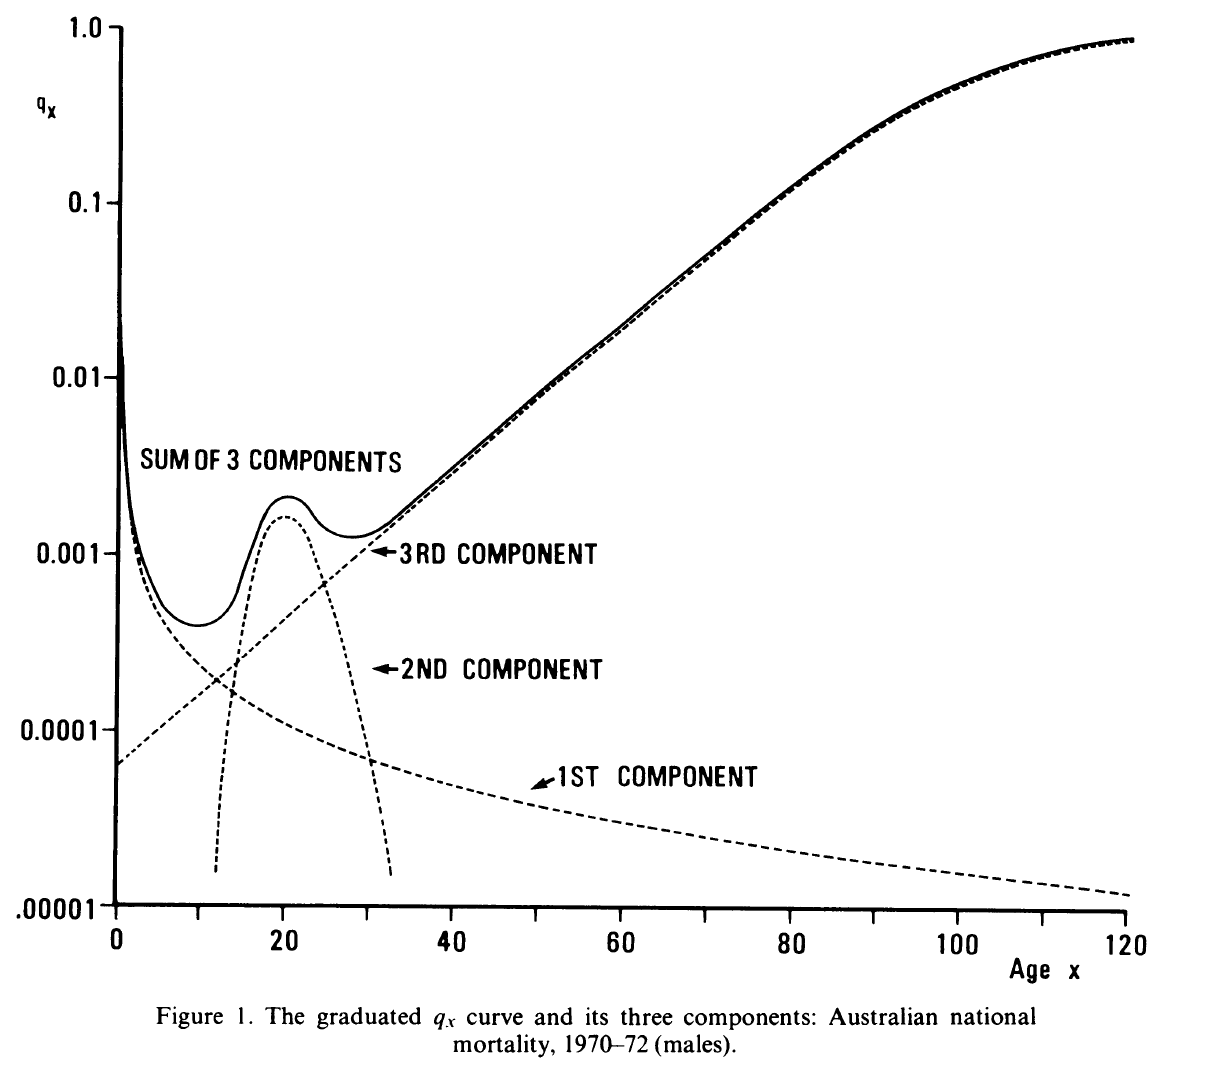
\includegraphics[width = 0.75\textwidth]{../figures/Helgman_pollard_model.png}
\caption{Illustration de l'impact de chacune des composantes du modèle de Heligman et Pollard.}
\label{fig:Helgman_pollard_model}
\end{figure}
\end{itemize}
La calibration de ces modèles se fait de deux façons
\begin{itemize}
  \item Par le maximum de vraisemblance sans utiliser les taux bruts
  \item Par les moindre carrés ordinaires, en minimisant l'écart entre les taux bruts et les taux du modèle paramétrique avec 
  $$
\argmax_{\theta\in\Theta}\sum_{x\geq 0}w_x(\widehat{q}_x - q_x(\theta))^2\text{ ou } \argmax_{\theta\in\Theta}\sum_{x\geq 0}w_x(\widehat{\mu}_x - \mu_x(\theta))^2
  $$
\end{itemize}
\begin{remark}
Pour le lissage des probabilité de décès, on peut par exemple choisir les poids inversement proportionnel de la variance des taux brut c'est à dire 
$$
w_x = \frac{E^0_x}{q_x(1-q_x)},\text{ ou }w_x = E_x^c \cdot\mu_x
$$
Cela va pénaliser les taux bruts aux grands âges.
\end{remark}
\subsection{Lissage non paramétrique}
Il est aussi possible de lisser la série des taux bruts sans faire d'hypothèse paramétrique. 
\subsubsection{Les moyennes mobiles}
La technique de lissage la plus simple consiste à prendre la moyenne des taux brut au voisinage de chaque âge. On remplace les taux bruts $\widehat{q}_x$ par 
$$
q^h_x = \sum_{k = -h}^h w_{x}^k \widehat{q}_x ,
$$
avec $w_x^k\geq 0,\text{ }k=-h,\ldots, h$ et $\sum_{k=-h}^{h} w_x^k = 1$ pour tout $x\geq 0$. Une façon naïve de choisir les poids consiste à prendre 
$$
w_x^k = \frac{1}{2h+1}.
$$
Une méthode plus élaborée fait intervenir un noyau de lissage $K:\RL_+\mapsto \RL_+$ qui est une fonction décroissante. Les taux lissé sont donné par 
$$
q^h_x = \sum_{y\geq0} \frac{K[(x-y)/h]}{\sum_{y\geq 0}K[(x-y)/h]}\widehat{q}_x.
$$
Les noyaux usuels incluent
\begin{itemize}
  \item Le noyau uniforme
  $$
K(u) = \frac{1}{2}\ind_{|u|<1}
  $$
  \item Le noyau triangle 
  $$
  K(u) = (1-|u|)\ind_{|u|<1}
  $$
  \item Le noyau Epanechnikov 
  $$
  K(u) = \frac{3}{4}(1-u^2)\ind_{|u|<1}
  $$
  \item Le noyau gaussien 
  $$
  K(u) = \frac{1}{\sqrt{2\pi}}\e^{-u^2/2}
  $$
\end{itemize}
Le lissage par noyau nécessite de choisir une fenêtre de lissage $h$.
\subsubsection{Le lissage de Whittaker-Henderson}
Le lissage de Whittaker-Henderson, expliqué par exemple dans le papier de \citet{Weinert2007}, consiste en un arbitrage entre la fidélité au taux brut $\widehat{q}_x$ et la régularité des taux lissés $\widehat{q}^\lambda_x$. Les taux lissés sont solution du problème d'optimisation 
$$
\argmax_{\widehat{q}^\lambda_x} \sum_{x=0}^{x^\ast}  F(\widehat{q}_x, q_x^\lambda) + \lambda R(q_x^\lambda),
$$
où $x^{\ast} = \sup \{x\in\mathbb{N}\text{ ; }q_x>0\}$ et $\lambda >0$ qui traduit le compromis entre fidélité $F$ et régularité $R$. Le critère de fidélité est donnée par 
$$
F(\widehat{q}_x, q_x^\lambda) = \sum_{x=0}^{x^\ast} w_x(\widehat{q}_x - q^{\lambda}_x)^2.
$$

le critère de régularité est donnée par 
$$
R(q_x) = \sum_{x=0}^{x^\ast-z} (\Delta^{z}q^\lambda_x)^2,
$$
où $\Delta^{z}q^\lambda_x$ est l'operateur de différence progressive d'ordre $z$ défini par 
$$
\Delta^{z}q^\lambda_x = \sum_{j=0}^z\binom{z}{j}(-1)^{z-j}q^\lambda_{x+j}.
$$
On note que 
$$
 \Delta^{1}q^\lambda_x = q^\lambda_{x+1}-q^\lambda_{x},\text{ }\Delta^{2}q^\lambda_x =\Delta^1 \Delta^1q^\lambda_x =q^\lambda_x q^\lambda_{x+2}-2q^\lambda_{x+1}+q^\lambda_{x},\ldots
$$
\begin{remark}
L'ordre $z$ de l'opréateur de différence progressive indique le niveau de lissage souhaité. Un polynôme de dégrée $z-1$ est ce que l'on peut obtenir de plus régulier. 
\begin{itemize}
  \item Pour $\lambda = 0$, on retrouve les taux bruts
  \item Pour $\lambda \rightarrow \infty$, on obtient le polynômes d'ordre $z-1$ qui ajuste le mieux la courbe des taux bruts suivant le critère des moindre carrés.
\end{itemize}
\end{remark}
L'implémentation passe par une représentation matricielle des différentes quantités. On a 
$$
W = \text{diag}\left( \begin{array}{ccc}w_1&\ldots&w_{x^\ast}\end{array}\right)\text{, }\widehat{q} = \left( \begin{array}{ccc}\widehat{q}_1&\ldots&\widehat{q}_{x^\ast}\end{array}\right)\text{, et }q^{\lambda} = \left( \begin{array}{ccc}q^{\lambda}_1&\ldots&q^{\lambda}_{x^\ast}\end{array}\right).
$$
Pour $z = 2$, on définit 
$$
K = \left(\begin{array}{cccccc}
-1&2&-1&0&\cdots&0\\
0&-1&2&-1&\cdots&0\\
\vdots&\ddots&\ddots&\ddots&\ddots&\vdots\\
0&\cdots&0&-1&2&-1\\
\end{array}\right).
$$
le problème d'optimisation devient 
$$
\argmin_{q^\lambda} \mathcal{L}(q^\lambda)= \argmin_{q^\lambda} \,^t(\widehat{q} - q^{\lambda})W(\widehat{q} - q^{\lambda})+\lambda\,^t(Kq^{\lambda})Kq^{\lambda}. 
$$
On en déduit que
$$
\frac{\text{d} }{\text{d} q^{\lambda}}\mathcal{L}(q^\lambda) =  2Wq^\lambda -2W\widehat{q}+2\lambda\,^tKKq^{\lambda}
$$
Le système d'équation 
$$
\frac{\text{d} }{\text{d} q^{\lambda}}\mathcal{L}(q^\lambda)=0
$$
a pour solution
$$
q^{\lambda} = \left(W + \lambda\,^tKK\right)^{-1}W\widehat{q}.
$$


\subsection{Fermeture de la table}
Le problème du manque (voir l'absence) de données aux grands âges oblige parfois d'avoir recours à des méthodes d'extrapolation. Deux méthodes sont décrites ci-après, l'idée est assez proche du lissage paramétrique. On utilise ces méthodes pour obtenir les $q_x$ aux grands âges. 

\subsubsection{Fermeture de Denuit-Goderniaux}
La méthode de \citet{Denuit2005} consiste à ajuster un modèle linéaire de la forme
$$
\log(\widehat{q}_x) = a + bx + cx^2+\epsilon_x,\text{ pour }x\in [x_{\min}, x_{\max}].
$$
où $\epsilon_x\overset{i.i.d.}{\sim}\NormalDist(0,\sigma^2)$. Les bornes $x_{\min}$ et $x_{\max}$ sont fixées de manière arbitraire par le modélisateur en fonction de la fiabilité des probabilités de décès aux grands âges. Deux conditions sont imposées
\begin{enumerate}
  \item la condition de fermeture $q_{130} = 1$
  \item la condition de concavité $q'_{130} = 0$. La probabilité de décès doit augmenter avec l'âge, cette croissance doit ralentir aux grands âges.
\end{enumerate}
Ces deux contraintes reviennent à imposer la relation suivante 
$$
a+bx+cx^2 = c(130-x)^2\text{, pour }x\in[x_{\min}, x_{\max}].
$$

\subsubsection{Fermeture de Kanisto}
La méthode de \citet{Thatcher1998} consiste à ajuster un modèle logistique de la forme
$$
\text{logit}(\widehat{q}_x) = \log\frac{q_x}{1-q_x}=\log(a) + bx,\text{ pour }x\in[x_{\min}, x_{\max}].
$$
par les moindre carrés ordinaires.
\begin{remark}
\begin{enumerate}
  \item L'ordre dans lequel on applique le lissage ou la fermeture est à la dsicrétion du praticien. On peut décider de lisser puis de fermer ou inversement. La fermeture peut entrainer une discontinuité dans la courbe d'où l'intérêt d'appliquer la procédure de lissage après la fermeture. L'utilisation de la fermeture sur les taux bruts peut nuire à l'estimation des paramètres d'où l'intérêt de lisser d'abord. On peut tout à fait lisser puis fermer et lisser à nouveau.
  \item La procédure de fermeture permet en premier lieu d'extrapoler les probabilités de décès aux âges non accessible. On peut également décider de remplacer les probabilités de décès des âges au dela de  $x_{\min}$ ou de  $x_{\max}$ ou encore prendre une moyenne entre taux brut et taux issus de la fermeture. Voir la note de la SOA\footnote{\url{https://www.soa.org/globalassets/assets/files/resources/essays-monographs/2005-living-to-100/m-li05-1-ix.pdf}}.
\end{enumerate}
\end{remark}
\section{Evolution temporelle de la mortalité et effet cohorte}
Les tables de mortalité générationnelles sont indexés sur l'année de calendaire $t$ à laquelle les données ont été recoltées ou l'année de naissance des individus $a= t-x$.
$$
\Data =  \bigcup_{t} \{E_{x,t}, D_{x,t}\}\text{ ou } \bigcup_{a} \{E_{x,a},D_{x,a}\}\text{ ou } \bigcup_{t,a} \{E_{x,t, a}, D_{x,t, a}\}
$$
On peut construire autant de table de mortalité "statique" que d'année calendaire ou de cohortes disponibles. Les tables générationelles TGH et TGF $05$ comprennent des projections permettant la traification des produits d'assurance vie. Ces tables prennent la forme de tableau à double entrée indexé sur l'âge et l'année de naissance, comme sur le \cref{tab:TGH05}.
\begin{table}[ht!]
\centering
\begin{tabular}{rrrrr}
  \hline
  Age & $1996$ & $1997$ & $1998$ &$\cdots$\\ 
  \hline
0 & 100000 & 100000 & 100000&$\cdots$ \\ 
 1 & 99607 & 99617 & 99626 &$\cdots$\\ 
 2 & 99487 & 99499 & 99510&$\cdots$ \\ 
 3 & 99435 & 99448 & 99460&$\cdots$ \\ 
 4 & 99406 & 99419 & 99432&$\cdots$ \\ 
$\vdots$ & $\vdots$ & $\vdots$ & $\vdots$&$\cdots$ \\ 
   \hline
\end{tabular}
\caption{Extrait de la table de mortalité générationnelle TGH $05$.}
\label{tab:TGH05}
\end{table}
La legislation impose l'utilisation de ces tables dans le cadre des contrats d'assurance vie comprenant des garanties du type rente viagère. On peut estimer les probabilités de décès par période $t_0\in[t, t+1]$ avec 
$$
q_{x,t_0} = \frac{d_{x,t_0}}{E_{x,t_0}},
$$
par génération $a_0\in[t-x, t-x+1]$ avec
$$
q_{x,a_0} = \frac{d_{x,a_0}}{E_{x,a_0}},
$$
ou par période et par cohorte avec
$$
q_{x,t_0, a_0} = \frac{d_{x,t_0, a_0}}{E_{x,t_0, a_0}},
$$
suivant le type de données disponibles. La construction des tables générationnelles à partir des données bruts nécessite l'introduction d'un outil graphique: le diagramme de Lexis.
\subsection{Diagramme de Lexis}
Le parcours des individus d'une population est représenté sur un diagramme de Lexis 
\begin{itemize}
\item Abscisse: $t = $ année calendaire ,
\item Ordonnée: $x=$ âge,
\end{itemize}
voir la \cref{fig:lexis}.
\begin{figure}
\begin{center}
\begin{tikzpicture}
\draw[->] (-1,0) -- (5,0);
\draw (5,0) node[right] {t};
\draw [->] (0,-1) -- (0,5);
\draw (0,5) node[above] {$x$};
\draw [dashed] (4,3) -- (0,3)  node[left] {$x_0$};
\draw [dashed] (4,3) -- (4,0) node[below] {$t_0$};
\draw [solid] (4,3) node{ \color{black}$\bullet$} -- (1,0) node[below] {$t_0-x_0$};
\end{tikzpicture}
\caption{Positionnement d'un individu qui décède à l'age $x_0$ durant l'année $t_0$ sur le diagramme de Lexis}
\label{fig:lexis}
\end{center}
\end{figure}
Lorsque les données sont exhaustives on peut représenter précisément le parcours de chaque individu sur le diagramme. 
\begin{figure}
\begin{center}
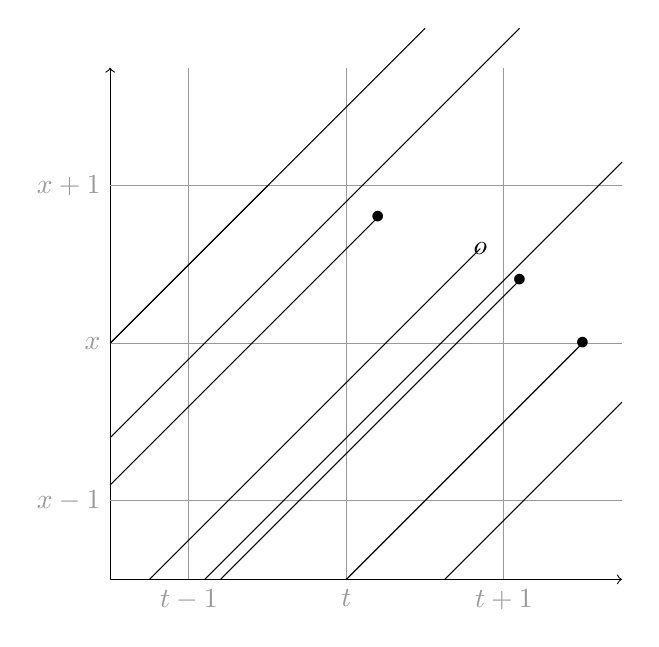
\begin{tikzpicture}
\draw[->] (0,0) -- (6.5,0);
\draw [->] (0,0) -- (0,6.5);
% Grid
\draw [color=gray!80] (1,0) node[below] {$t-1$} -- (1,6.5);
\draw [color=gray!80] (3,0) node[below] {$t$} -- (3,6.5);
\draw [color=gray!80] (5,0) node[below] {$t+1$} -- (5,6.5);
\draw [color=gray!80] (0,1) node[left] {$x-1$} -- (6.5,1);
\draw [color=gray!80] (0,3) node[left] {$x$} -- (6.5,3);
\draw [color=gray!80] (0,5) node[left] {$x+1$} -- (6.5,5);
% 
\draw plot[domain=0:4] (\x, 3+\x);
\draw plot[domain=0:5.2] (\x, 1.8+\x);
\draw plot[domain=0:3.4] (\x, 1.2+\x) node[] {$\bullet$};
\draw plot[domain=0.5:4.7] (\x, -0.5+\x) node[] {$o$};
\draw plot[domain=1.2:6.5] (\x, -1.2+\x) node[] {};
\draw plot[domain=1.4:5.2] (\x, -1.4+\x) node[] {$\bullet$};
\draw plot[domain=3:6] (\x, -3+\x) node[] {$\bullet$};
\draw plot[domain=4.25:6.5] (\x, -4.25+\x) node[] {};
\draw plot[domain=0:2] (\x, 3+\x) ;
\end{tikzpicture}
\caption{Parcours des individus sur le diagramme de Lexis. $\bullet=$  décès et $o=$ fin d'observation de l'individu (censure à droite)}
\label{fig:lexis}
\end{center}
\end{figure}
l'estimation des taux de mortalité se résume à compter le nombre de décès ($\bullet$) dans les triangles, les carrés ou les parallélogramme du diagramme de Lexis suivant que l'on calcule des taux de décès pour
\begin{itemize}
  \item une période $t_0\in[t, t+1)$: carré de Lexis
  \item cohorte $a_0\in[t-x, t-x+1)$: parallélogramme de Lexis
  \item période et cohorte $(t_0,a_0)\in[t, t+1)\times [t-x, t-x+1)$: triangle de Lexis
\end{itemize}

puis à rapporter ce nombre sur l'exposition au risque. Lorsque l'on connait la date exacte des décès, l'exposition est le cumul des longueurs des segments des parcours passant au travers du carré, triangle ou parallélogramme étudié, voir la \cref{fig:lexis_geom}. 
\begin{figure}[ht!]
\begin{center}
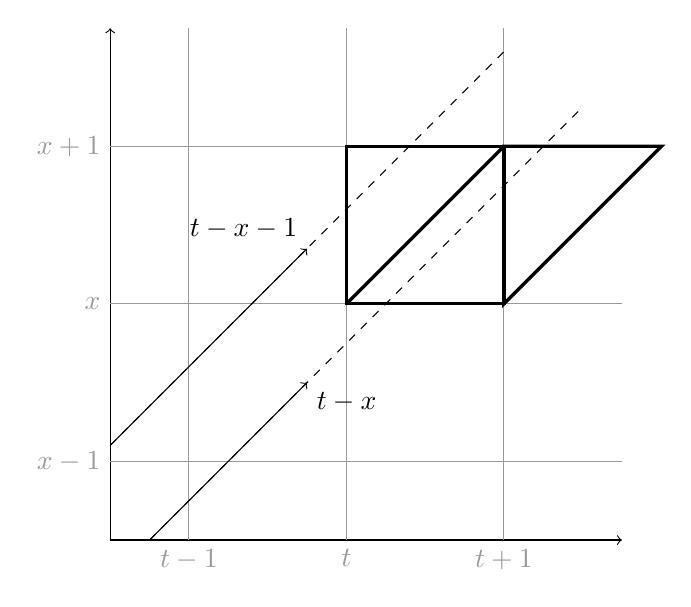
\begin{tikzpicture}
\draw[->] (0,0) -- (6.5,0);
\draw [->] (0,0) -- (0,6.5);
% Grid
\draw [color=gray!80] (1,0) node[below] {$t-1$} -- (1,6.5);
\draw [color=gray!80] (3,0) node[below] {$t$} -- (3,6.5);
\draw [color=gray!80] (5,0) node[below] {$t+1$} -- (5,6.5);
\draw [color=gray!80] (0,1) node[left] {$x-1$} -- (6.5,1);
\draw [color=gray!80] (0,3) node[left] {$x$} -- (6.5,3);
\draw [color=gray!80] (0,5) node[left] {$x+1$} -- (6.5,5);
% 

\draw[-, dashed] plot[domain=0:5] (\x, 1.2+\x)  node[above left] {};
\draw[->] plot[domain=0:2.5] (\x, 1.2+\x)  node[above left] {$t-x-1$};
\draw[-,, dashed] plot[domain=0.5:6] (\x, -0.5+\x) node[below right] {};
\draw[->] plot[domain=0.5:2.5] (\x, -0.5+\x) node[below right] {$t-x$};
\draw [-, very thick] (3,3) -- (5,5);
\draw [very thick] (3,3) -- (3,5) -- (5,5) -- (5,3) -- cycle;
\draw [very thick] (5,3) -- (5,5) -- (7,5) -- cycle;
\end{tikzpicture}
\caption{Géométrie de Lexis}
\label{fig:lexis_geom}
\end{center}
\end{figure}
Les individus de la cohorte nés l'année $t-x$ atteindrons l'âge $x$ durant les années calendaires $t$ et $t+1$.
\begin{remark}
L'estimateur prenant en compte la longueur de segment pour le calcul de l'exposition est l'estimateur de \citet{Hoem1971}. Il est très utilisé en sciences actuarielle, une comparaison avec l'estimateur de Kaplan-Meier dans le cadre d'une application à la mortalité est proposé dans \citet{Guibert2017}. La méthodologie ci-après suit le protocole de calcul établi dans le cadre du projet HMD\footnote{\url{https://www.mortality.org/}} voir \citet{Wilmoth2007}. 
\end{remark}
\subsection{Taux de mortalité par période}
Considérons les évènements se produisant sur la période $[t, t+1]$, nous intéressons au carré de Lexis de la \cref{fig:lexis_square}
\begin{figure}
\begin{center}
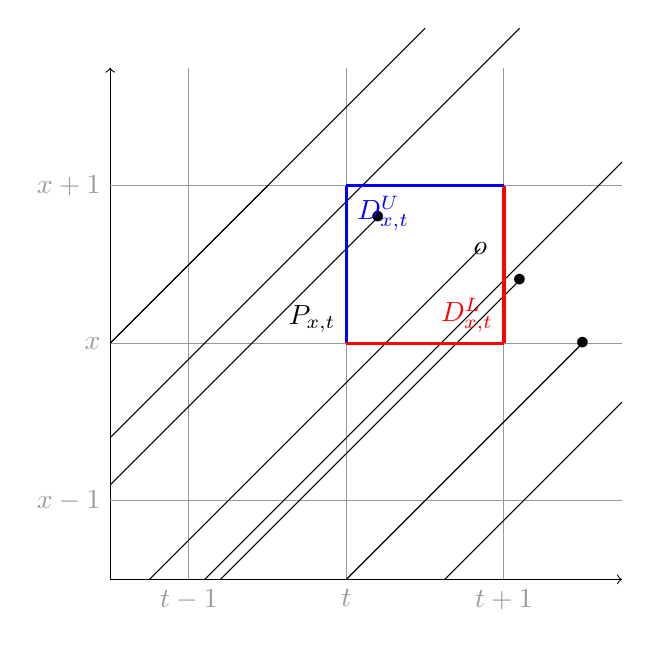
\begin{tikzpicture}
\draw[->] (0,0) -- (6.5,0);
\draw [->] (0,0) -- (0,6.5);
% Grid
\draw [color=gray!80] (1,0) node[below] {$t-1$} -- (1,6.5);
\draw [color=gray!80] (3,0) node[below] {$t$} -- (3,6.5);
\draw [color=gray!80] (5,0) node[below] {$t+1$} -- (5,6.5);
\draw [color=gray!80] (0,1) node[left] {$x-1$} -- (6.5,1);
\draw [color=gray!80] (0,3) node[left] {$x$} -- (6.5,3);
\draw [color=gray!80] (0,5) node[left] {$x+1$} -- (6.5,5);
% 
\draw plot[domain=0:4] (\x, 3+\x);
\draw plot[domain=0:5.2] (\x, 1.8+\x);
\draw plot[domain=0:3.4] (\x, 1.2+\x) node[] {$\bullet$};
\draw plot[domain=0.5:4.7] (\x, -0.5+\x) node[] {$o$};
\draw plot[domain=1.2:6.5] (\x, -1.2+\x) node[] {};
\draw plot[domain=1.4:5.2] (\x, -1.4+\x) node[] {$\bullet$};
\draw plot[domain=3:6] (\x, -3+\x) node[] {$\bullet$};
\draw plot[domain=4.25:6.5] (\x, -4.25+\x) node[] {};
\draw plot[domain=0:2] (\x, 3+\x) ;
\draw [blue, very thick] (3,3) node[above left] {\color{black} $P_{x,t}$}   -- (3,5) ;
\draw [red, very thick] (3,3) -- (5,3) node[above left] {\color{red}$ D^L_{x,t}$};
\draw [red, very thick] (5,5) -- (5,3)  ;
\draw [blue, very thick] (3,5) node[below right] {\color{blue}$D^U_{x,t}$}  -- (5,5)  ;
 % --  -- cycle;
\end{tikzpicture}
\caption{Parcours des individus sur le diagramme de Lexis. $\bullet=$  décès et $o=$ fin d'observation de l'individu (censure à droite)}
\label{fig:lexis_square}
\end{center}
\end{figure}
\begin{itemize}
\item $P_{x,t} = 2$ est le nombre d'individu d'âge $x$ au début de la périod $t$. Il s'agit du nombre de segment intersectant le côté $(x,t) - (t,x+1)$.
\item $D^U_{x,t}=1$ compte le nombre de décès d'individu d'âge $x$ au début de la période $[t, t+1]$
\item $D^L_{x,t}=0$ compte le nombre de décès d'individu d'âge atteignant l'âge $x$ durant la période $[t, t+1]$.
\item Le nombre de décès au cours de la période est donné par 
$$
D_{x,t} = D^U_{x,t} + D^L_{x,t} = 1.
$$
\end{itemize} 
L'exposition exacte est donnée par la somme des longueurs des segments dans le carré de Lexis, ici 
$$
E_{x,t} =  0.08 + 0.3 + 0.6 + 0.42 + 0.33 = 1.73.
$$
La probabilité de décès d'un individu d'âge $x$ durant la période $[t, t+1]$ est égale à 
$$
q_{x,t} = \frac{1}{1.73} = 0.57.
$$
Si les longueurs de segments ne sont pas accessible l'exposition est approchée en sommant l'exposition des trianges supérieurs et inférieur avec 
$$
E_{x,t} = E_{x,t}^L + E_{x,t}^U.
$$
L'exposition du triangle inférieur comprend $P_{x,t+1}$ la population d'âge $x$ au début de l'année $t+1$ auquel nous devons ajouter la contribution des décès du triangle inférieur. On a 
$$
E_{x,t}^L = l_1P_{x,t+1}+l_2D^{L}_{x,t}.
$$
L'exposition du triangle supérieur comprend $P_{x,t}$ la population d'âge $x$ au début de l'année $t$ à laquelle nous devons soustraire la contribution des décès du triangle supérieur.  
$$
E_{x,t}^U = u_1P_{x,t}-u_2D^{U}_{x,t}.
$$
Les coefficients l$_1, l_2, u_1$ et $u_2$ peuvent être inférés à l'aide de la distribution des naissance pour les cohortes $t-x-1$ et $t-x$ comme sur la \cref{fig:Lexis_expo_computation}. 
\begin{figure}[h!] 
\centering
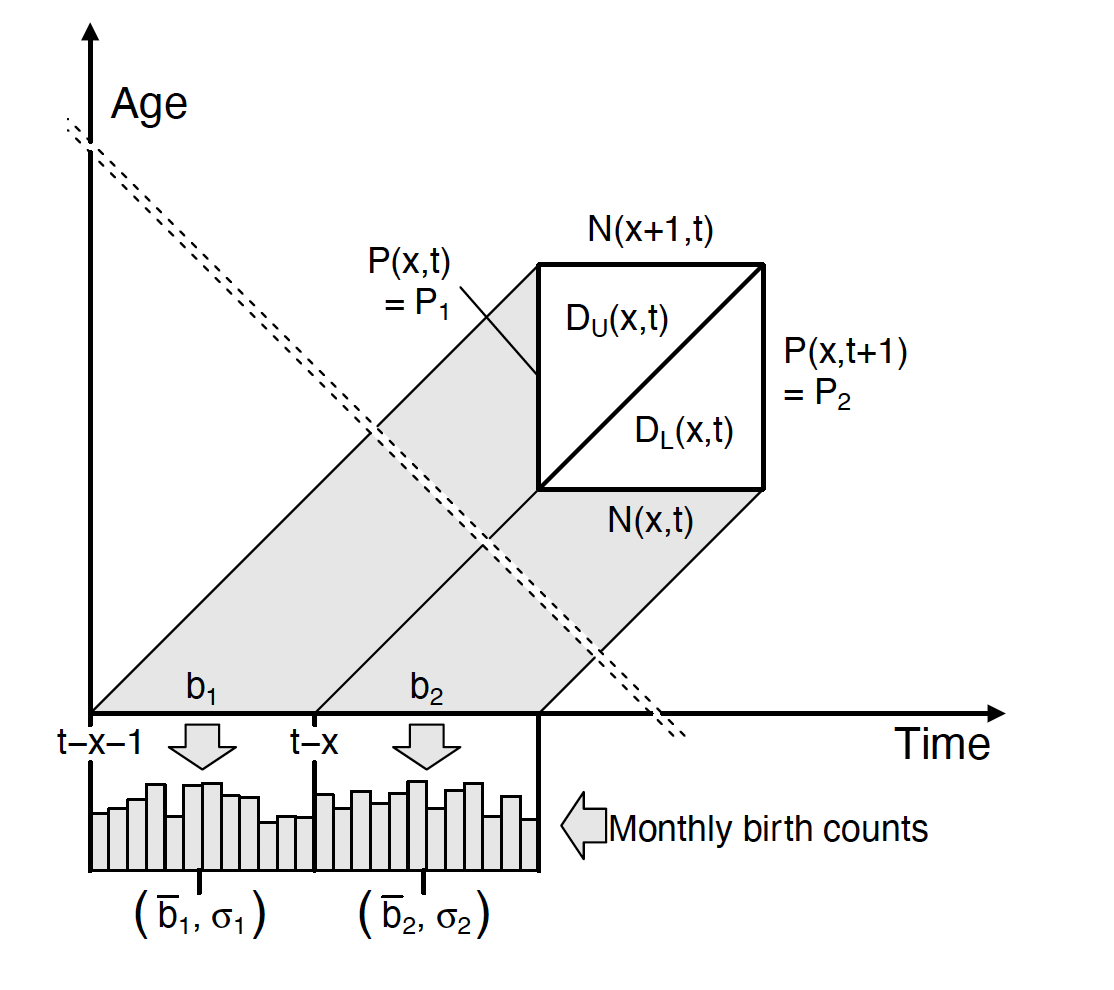
\includegraphics[width = 0.75\textwidth]{../figures/Lexis_expo_computation.png}
\caption{Calcul d'exposition central sur un diagrame de Lexis grâce à la distribution des naissances pour les cohortes concernées. (Source: HMD Documentation)}
\label{fig:Lexis_expo_computation}
\end{figure}
Soit $B_1,B_2\in[0,1]$ les \va qui indiquent la répartition des naissances au sein de la cohorte $t-x-1$ et $t-x$ respectivement. Soient $f_{B_1}$ et $f_{B_2}$ les densités de $B_1$ et $B_2$. On note également 
$$
\bar{b}_i = \E(B_i),\text{ et }\sigma_i^2 = \V(B_i),\text{ pour }i = 1,2.
$$
Dans le triangle inférieur, la contribution à l'exposition des individus d'âge $x$ au temps $t+1$ est donnée par 
\begin{equation}\label{eq:expos_contribution_lower}
\E\left[1-B_2\right] = (1-\bar{b}_2), 
\end{equation}
Dans le triangle supérieur, la contribution des individus d'âge $x$ à l'année $t$ à l'exposition  est donnée par 
\begin{equation}\label{eq:expos_contribution_upper}
\E\left(B_1\right)=\bar{b}_1.
\end{equation}
La contribution des décès est un peu plus subtil. Un décès dans le triangle inférieur est un point $(t+U, x+V)$ avec $(U,V)$ un couple de variable aléatoire telle que $0\leq V\leq U\leq 1$. On suppose que la densité jointe de $(U,V)$ est donnée par 
\begin{equation}\label{eq:joint_density_lower}
f_{(U,V)}(u,v) = C_L f_{B_{2}}(u-v)\mathbb{I}_{0\leq v\leq u\leq 1}(u,v),
\end{equation}
où $C_L$ est une constante de normalisation. Ce choix entraine que 
\begin{itemize}
  \item La probabilité que le décès survienne est constante le long de la ligne de vie
  \item La densité est proportionelle à la densité de probabilité de $B_2$
\end{itemize}
En intégrant \eqref{eq:joint_density_lower}, on identifie $C_L = 1/(1-\bar{b}_{2})$. Pour un décès qui a lieu au point $(t+U, x+V)$, la perte d'exposition est donnée par 
\begin{equation}\label{eq:lost_exposure_death_lower}
\int_{0}^1\int_{0}^u(1-u)f_{B_2}(u-v)\text{d}v\text{d}u = \frac{1-\bar{b}_2}{2}+\frac{\sigma_2^2}{2(1-\bar{b}_2)}
\end{equation}
On déduit de \eqref{eq:expos_contribution_lower} et \eqref{eq:lost_exposure_death_lower} l'exposition dans le triangle inférieur avec 
\begin{eqnarray*}
E^L_{x,t}&=&(1-\bar{b}_2)(P_{x,t+1}+D^L_{x,t}) - \left(\frac{1-\bar{b}_2}{2}+\frac{\sigma_2^2}{2(1-\bar{b}_2)}\right)D^L_{x,t}\\
& =& (1-\bar{b}_2)P_{x,t+1} + \left(\frac{1-\bar{b}_2}{2}-\frac{\sigma_2^2}{2(1-\bar{b}_2)}\right)D^L_{x,t}\\
&=& l_1P_{x,t+1} + l_2 D^L_{x,t}
\end{eqnarray*}
Un décès dans le triangle supérieur est un point $(t+U, x+ V)$ avec $0\leq U\leq V\leq 1$. La densité jointe de $(U,V)$ est donnée par (pour les mêmes raison que précédemment)
\begin{equation}\label{eq:joint_density_upper}
f_{(U,V)}(u,v) = C_U f_{B_{1}}(u+1-v)\mathbb{I}_{0\leq u\leq v\leq 1}(u,v),
\end{equation}
En intégrant \eqref{eq:joint_density_upper}, on identifie $C_U = 1/\bar{b}_{1}$. Pour un décès qui a lieu au point $(t+U, x+V)$, la perte d'exposition est donnée par 
\begin{equation}\label{eq:lost_exposure_death_upper}
\int_{0}^1\int_{u}^1uf_{B_2}(u+1-v)\text{d}v\text{d}u = \frac{\bar{b}_1}{2}+\frac{\sigma_2^2}{2\bar{b}_1}
\end{equation}
On déduit de \eqref{eq:expos_contribution_upper} et \eqref{eq:lost_exposure_death_upper} l'exposition dans le triangle inférieur avec 
\begin{eqnarray*}
E^U_{x,t}&=&\bar{b}_1(P_{x,t}-D^U_{x,t}) + \left(\frac{\bar{b}_1}{2}+\frac{\sigma_1^2}{2\bar{b}_1}\right)D^U_{x,t}\\
& =& \bar{b}_1P_{x,t} - \left(\frac{\bar{b}_1}{2}-\frac{\sigma_1^2}{2\bar{b}_2}\right)D^U_{x,t}\\
&=& u_1P_{x,t} - u_2 D^U_{x,t}
\end{eqnarray*}

En l'absence d'information sur la distribution des naissances au cours des l'années au sein des cohortes, on suppose que $B_1,B_2\sim\UnifDist(0,1)$. Il vient alors
$$
E_{x,t} \approx  \frac{1}{2}[P_{x,t}+ P_{x,t+1}] + \frac{1}{6}[D^L_{x,t}- D^U_{x,t}] = 1.7.
$$
La probabilité de décès d'un individu d'âge $x$ durant la période $[t, t+1]$ est égale à 
$$
\widehat{q}_{x,t} = \frac{1}{1.7} = 0.59.
$$
\begin{remark}
Si nous n'avons accès qu'au nombre de décès $D_{x,t}$ d'individus d'âge $x$ pendant l'année $t$ alors on peut considérer que $D^U_{x,t} = D^L_{x,t} = D_{x,t} / 2$. Pour plus de détail sur les calculs d'exposition en prenant en compte les données de natatlité, voir le travail de \citet{Boumezoued2020}.
\end{remark}
\subsection{Taux de mortalité par cohorte}
Considérons les évènements concernant les individus d'âge $x$ nés l'année $a=t-x$, nous intéressons au parallélogramme de Lexis de la \cref{fig:lexis_para}
\begin{figure}
\begin{center}
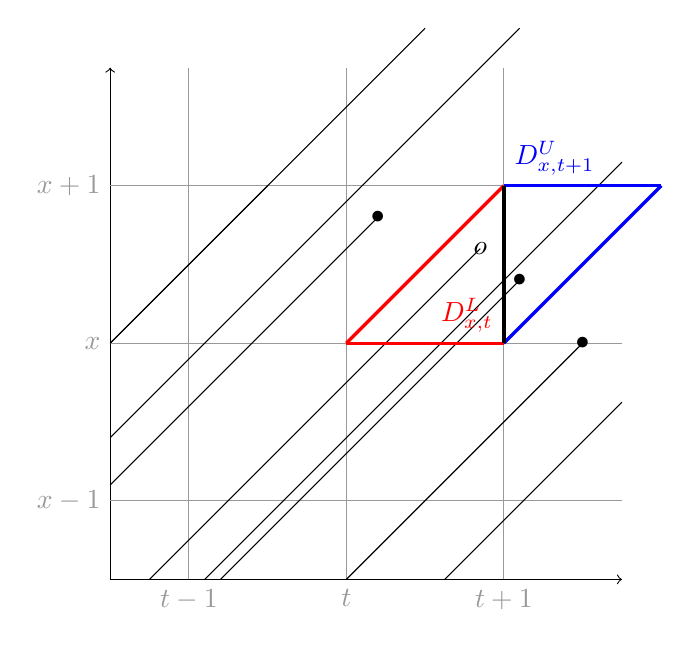
\begin{tikzpicture}
\draw[->] (0,0) -- (6.5,0);
\draw [->] (0,0) -- (0,6.5);
% Grid
\draw [color=gray!80] (1,0) node[below] {$t-1$} -- (1,6.5);
\draw [color=gray!80] (3,0) node[below] {$t$} -- (3,6.5);
\draw [color=gray!80] (5,0) node[below] {$t+1$} -- (5,6.5);
\draw [color=gray!80] (0,1) node[left] {$x-1$} -- (6.5,1);
\draw [color=gray!80] (0,3) node[left] {$x$} -- (6.5,3);
\draw [color=gray!80] (0,5) node[left] {$x+1$} -- (6.5,5);
% 
\draw plot[domain=0:4] (\x, 3+\x);
\draw plot[domain=0:5.2] (\x, 1.8+\x);
\draw plot[domain=0:3.4] (\x, 1.2+\x) node[] {$\bullet$};
\draw plot[domain=0.5:4.7] (\x, -0.5+\x) node[] {$o$};
\draw plot[domain=1.2:6.5] (\x, -1.2+\x) node[] {};
\draw plot[domain=1.4:5.2] (\x, -1.4+\x) node[] {$\bullet$};
\draw plot[domain=3:6] (\x, -3+\x) node[] {$\bullet$};
\draw plot[domain=4.25:6.5] (\x, -4.25+\x) node[] {};
\draw plot[domain=0:2] (\x, 3+\x) ;
\draw [blue, very thick] (5,5) node[above right] {\color{blue}$D^U_{x,t+1}$} -- (7,5);
\draw [blue, very thick] (5,3)-- (7,5);
\draw [red, very thick] (3,3) -- (5,3) node[above left] {\color{red}$ D^L_{x,t}$};
\draw [red, very thick] (3,3) -- (5,5) ;
\draw [black, very thick] (5,5) -- (5,3) ;
% \draw [blue, very thick] (3,5)   -- (5,5)  ;
 % --  -- cycle;
\end{tikzpicture}
\caption{Parcours des individus sur le diagramme de Lexis. $\bullet=$  décès et $o=$ fin d'observation de l'individu (censure à droite)}
\label{fig:lexis_para}
\end{center}
\end{figure}
L'exposition est donnée par la somme des longueurs des segments dans le parallélogramme, soit 
$$
E_{x,a} = 0.8+1+0.4 =2.2.
$$
La probabilité de décès des individus d'âge $x$ né l'année $a$ est donnée par 
$$
q_{x,a} = 1/2.2 = 0.45.
$$

Si la longueur des segments est inconnue alors au vu des calculs effectués pour les taux de mortalité par période, il vient
$$
E_{x,a}= P_{x,t+1} + \left(\frac{1-\bar{b}}{2}+\frac{\sigma^2}{2(1-\bar{b})}\right)D^L_{x,t} -  \left(\frac{\bar{b}}{2}+\frac{\sigma^2}{2\bar{b}}\right)D^U_{x,t+1}
$$
avec $a =t-x$, voir \cref{fig:death_rate_cohort_HMD}.
\begin{figure}[h!] 
\centering
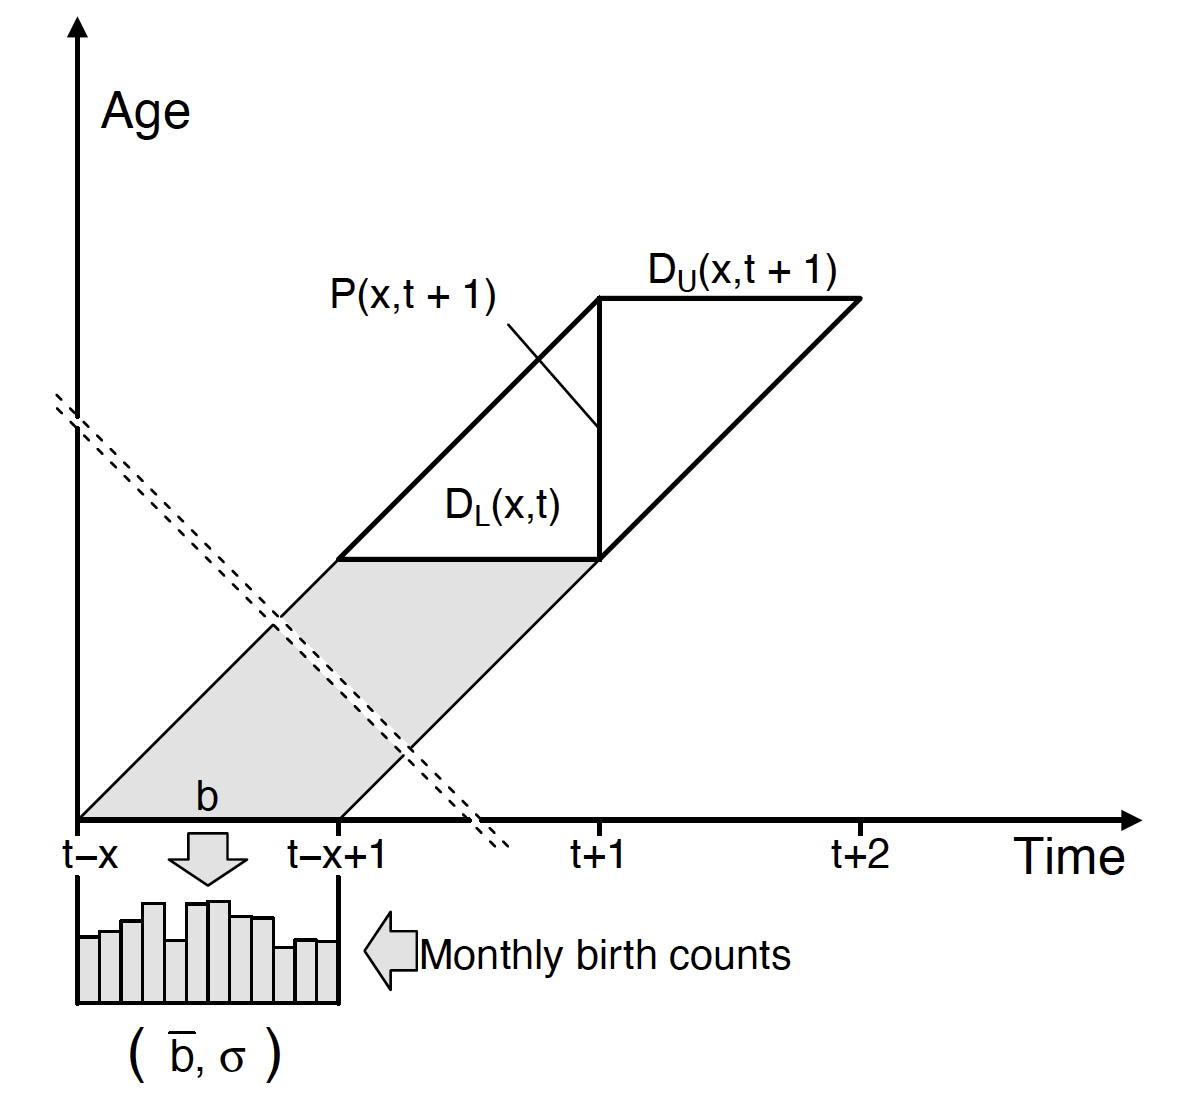
\includegraphics[width = 0.75\textwidth]{../figures/death_rate_cohort_HMD.png}
\caption{Calcul d'exposition central sur un diagrame de Lexis grâce à la distribution des naissances pour la cohortes concernée. (Source: HMD Documentation)}
\label{fig:death_rate_cohort_HMD}
\end{figure}
Si l'information sur les moments de la distribution des naissances n'est pas disponible alors on suppose une distribution uniforme qui mène à la simplification suivante 
$$
E_{x,a}= P_{x,t+1} + \frac{1}{3}(D^L_{x,t} - D^U_{x,t+1})
$$
puis
$$
\widehat{q}_{x,a} = 1/2 = 0.5.
$$ 
% \subsection{Taux de décès par période et cohorte}
% Considérons les évènements concernant les individus d'âge $x$,  nés l'année $a=t-x$, durant la période $[t,t+1]$. Nous nous intéressons au triangle de Lexis de la \cref{fig:lexis_triangle}
% \begin{figure}
% \begin{center}
% \begin{tikzpicture}
% \draw[->] (0,0) -- (6.5,0);
% \draw [->] (0,0) -- (0,6.5);
% % Grid
% \draw [color=gray!80] (1,0) node[below] {$t-1$} -- (1,6.5);
% \draw [color=gray!80] (3,0) node[below] {$t$} -- (3,6.5);
% \draw [color=gray!80] (5,0) node[below] {$t+1$} -- (5,6.5);
% \draw [color=gray!80] (0,1) node[left] {$x-1$} -- (6.5,1);
% \draw [color=gray!80] (0,3) node[left] {$x$} -- (6.5,3);
% \draw [color=gray!80] (0,5) node[left] {$x+1$} -- (6.5,5);
% % 
% \draw plot[domain=0:4] (\x, 3+\x);
% \draw plot[domain=0:5.2] (\x, 1.8+\x);
% \draw plot[domain=0:3.4] (\x, 1.2+\x) node[] {$\bullet$};
% \draw plot[domain=0.5:4.7] (\x, -0.5+\x) node[] {$o$};
% \draw plot[domain=1.2:6.5] (\x, -1.2+\x) node[] {};
% \draw plot[domain=1.4:5.2] (\x, -1.4+\x) node[] {$\bullet$};
% \draw plot[domain=3:6] (\x, -3+\x) node[] {$\bullet$};
% \draw plot[domain=4.25:6.5] (\x, -4.25+\x) node[] {};
% \draw plot[domain=0:2] (\x, 3+\x) ;
% % \draw [blue, very thick] (5,5) node[below right] {\color{blue}$D^U_{x,t}$} -- (7,5);
% % \draw [blue, very thick] (5,3)-- (7,5);
% \draw [red, very thick] (3,3) -- (5,3) node[above left] {\color{red}$ D^L_{x,t}$};
% \draw [red, very thick] (3,3) -- (5,5) ;
% \draw [red, very thick] (5,5) -- (5,3) ;
% % \draw [blue, very thick] (3,5)   -- (5,5)  ;
%  % --  -- cycle;
% \end{tikzpicture}
% \caption{Parcours des individus sur le diagramme de Lexis. $\bullet=$  décès et $o=$ fin d'observation de l'individu (censure à droite)}
% \label{fig:lexis_triangle}
% \end{center}
% \end{figure}
% L'exposition est donnée par la somme des longueurs des segments dans le triangle, soit 
% $$
% L^c(x,a) \approx 0.8 + 0.4 + 0.3 = 1.5
% $$
% La probabilité de décès des individus d'âge $x$ né l'année $a$ est donnée par 
% $$
% q_{x,a} = 0/1.5 = 0.
% $$
% Si la longueur des segments est inconnue alors on fait l'approximation suivante 
% $$
% L^c(x,a) \approx L_{x,t+1} - \frac{1}{2}D^L_{x,t}  = 2
% $$
% et
% $$
% \widehat{q}_{x,a} = 0/2 = 0.
% $$ 
\subsection{Modèle de projection de la mortalité}
L'objectif est de rendre compte de la tendance des taux de mortalité $\mu_{x,t}$ et probabilités de décès $q_{x,t}$ au cours du temps. Dans la section précédente, nous avons estimé des expositions dites centrales $E_{x,t}^c$. Les taux de mortalités sont estimés sur la base de l'exposition centrale avec 
$$
\mu_{x,t} = \frac{D_{x,t}}{E_{x,t}^c}.
$$
Les probabilité de décès requiert usuellement l'exposition initiale $E_{x,t^0}$ avec 

$$
q_{x,t} = \frac{D_{x,t}}{E_{x,t}^0}.
$$
Les deux expositions sont approximativement lié par $E_{x,t}^0\approx E_{x,t}^c +D_{x,t}/2$. On utilisera la notation $E_{x,t}$ pour l'exposition centrale ou initiale lorsque le contexte est clair. Les probabilité de décès et taux de mortalité sont liés par
$$
q_{x,t}=1-\exp(-\mu_{x,t}).
$$
Les modèles de mortalité stochastique, aussi appelé GAPC (\textit{Generalized} Age-Period-Cohort comprennent $4$ composantes.
\begin{enumerate}  
  \item Une composante aléatoire  
  $$
D_{x,t}\sim \PoissonDist(\mu_{x,t}\cdot E_{x,t}^c)\text{, avec }\E(D_{x,t}) = E_{x,t}^c\cdot \mu_{x,t},
  $$
  ou
  $$
D_{x,t}\sim \BinomialDist( E_{x,t}^0, q_{x,t})\text{, avec }\E(D_{x,t}) = E_{x,t}^0\cdot q_{x,t},
  $$
  \item Une composante systématique
  $$
\eta_{x,t} = \alpha_x + \sum_{i=1}^N \beta_{x}^{(i)}\kappa_{t}^{(i)}+\beta_{x}^{(0)}\gamma_{t-x},
  $$
  où
  \begin{itemize}
    \item Le terme $\alpha_x$ caractérise l'effet statique de l'âge sur la mortalité
    \item $N$ est le nombre de terme de type age-période. Les termes $\kappa_t^{(i)},\text{ }i=1,\ldots, N$ décrivent la tendance de la mortalité au cours du temps modulé par l'âge via les termes $\beta_x^{(i)}$
    \item Le terme $\gamma_{t-x}$ tient compte d'un possible effet cohorte modulé par l'âge via le terme $\beta_{x}^{(0)}$.
  \end{itemize}
  Les termes age-dépendant $\beta_x^{i}$ peuvent être des fonctions prédeterminé de l'âge $\beta_x^{i} = f^{i}(x)$ ou bien des coefficients sans structures préalables. Les termes périodes-dépendant $\kappa_t^{i}$ et cohortes-dépendants $\gamma_{t-x}$ sont considérés comme des processus stochastiques. Les méthodes d'études des série chronologiques s'appliquent pour effectuer les prévisions de l'évolution de la mortalité. Cette structure permet de prendre en compte la plupart des modèles de mortalités, voir \citet{Hunt2020}.
  \item La fonction de lien $g$ entre la composante aléatoire et la composante systématique avec 
  $$
  g\left[\E\left(\frac{D_{x,t}}{E_{x,t}}\right)\right] =  \eta_{x,t}.
  $$
  Dans le cadre du modèle de Poisson, on utilise la fonction log\footnote{$\log(\mu_{x,t})$}. Pour le modèle binomial la fonction logit\footnote{$\log(q_{x,t}/(1-q_{x,t}))$}. Ce sont les fonctions de lien canonique des modèles linéaires généralisés, voir \citet{Currie2014} pour une discussion sur les fonctions de liens dans le cadre des modèles de mortalités stochastiques.
  \item Les contraintes sur les paramètres permettant de rendre le modèle identifiable. On applique au vecteur de paramètres
  $$
  \theta = \left(\alpha_x,\beta_{x}^{(1)},\ldots, \beta_x^{(N)},\kappa_{t}^{(1)},\ldots, \kappa_{t}^{(N)}, \beta^{(0)}, \gamma_{t-x}\right)
  $$
  une transformation $v$ avec 
$$
  \tilde{\theta} = \left(\tilde{\alpha}_x,\tilde{\beta}_{x}^{(1)},\ldots, \tilde{\beta}_x^{(N)},\tilde{\kappa}_{t}^{(1)},\ldots, \tilde{\kappa}_{t}^{(N)}, \tilde{\beta}^{(0)}, \tilde{\gamma}_{t-x}\right).
$$
La conséquence est une perte de degré de liberté sans changer le prédicteur $\eta_{x,t}$.
\end{enumerate}

\begin{ex}
Voici quelques exemples de modèles de type GAPC.
\begin{enumerate}
  \item Dans le modèle de \citet{Lee1992}, on utilise le modèle de Poisson et le prédicteur est donnée par 
  $$
  \eta_{x,t} = \alpha_x +\beta_x\kappa_t.
  $$
  La composante temporelle est modélisée par une marche aléatoire avec une tendance, c'est à dire 
  $$
  \kappa_t = \delta + \kappa_{t-1}+ \epsilon_t,\text{ avec }\epsilon_t\sim\NormalDist(0,\sigma^2).
  $$
  Le modèle de Lee-Carter n'est pas identifiable au sens où la transformation 
  $$
  (\alpha_x\text{, }\beta_x\text{, }\kappa_t)\mapsto\left(\alpha_x + c_1\beta_x\text{, } \frac{\beta_x}{c_2}\text{, } c_2(\kappa_t-c_1)\right)
  $$
  n'a aucun effet sur les $\eta_{x,t}$. On impose donc les conditions suivante 
  $$
  \sum_x \beta_x=1 \text{ et }\sum_t\kappa_t =0,
   $$
   ce qui revient à fixer $c_1$ et $c_2$ de la façon suivante
   $$
   c_1=\frac{1}{n}\sum_{t}\kappa_t\text{, et }c_2 = \sum_x\beta_x,
   $$
   où $n$ est le nombre d'année d'historique.
  \item Le modèle APC, voir \citet{Clayton1987}, s'appuie aussi sur le modèle de Poisson et suppose que 
  $$
  \eta_{x,t}= \alpha_x + \kappa_t + \gamma_{t-x}.
  $$
  Le modèle APC n'est pas identifiable car il est invariant par rapport aux deux transformations suivantes
  $$
  (\alpha_x\text{, }\text{, }\kappa_t\text{, }\gamma_{t-x})\mapsto\left(\alpha_x + \phi_1-\phi_2x\text{, } \kappa_t+\phi_2 t\text{, } \gamma_{t-x}-\phi_1 - \phi_2(t-x)\right)
  $$
  et 
  $$
  (\alpha_x\text{, }\kappa_t\text{, }\gamma_{t-x})\mapsto\left(\alpha_x + c_1\text{, } \kappa_t-c_1\text{, } \gamma_{t-x}\right),
  $$
  où $c_1,\phi_1$ et $\phi_2$ sont des constantes dans $\RL$. L'identifiabilité est obtenue en imposant les contraintes suivantes
  $$
\sum_{t}\kappa_t = 0\text{, }\sum_{a=t_1-x_k}^{t_n-x_1}\gamma_a=0\text{, }\sum_{a=t_1-x_k}^{t_n-x_1}a\gamma_a=0,
$$
où $x_1 = \min x$, $t_1=\min t$, $x_k = \max x$ et $t_n = \max t_n$. L'effet cohorte fluctue autour de $0$ sans faire apparaître de tendance. Les contraintes sont imposées d'abord par une regression linéaire de $\gamma_{t-x}$ sur $t-x$ avec 
$$
\gamma_{t-x} = \phi_1 + \phi_2(t-x) + \epsilon_{t-x},\text{ }\epsilon_{t-x}\sim\NormalDist(0,\sigma^2).
$$
puis la contrainte sur la composante temporelle
$$
c_1 = \frac{1}{n}\sum_t\kappa_t,
$$
\item Le modèle CBD de \citet{Cairns2006} s'appuie sur le modèle binomiale et un prédicteur donné par 
$$
\eta_{x,t} = \kappa_t^{(1)} + (x-\bar{x})\kappa_t^{(2)}.
$$
Les composantes temporelles sont modélisés par une marche aléatoire bivariée. Ce modèle est identifiable donc aucune contrainte n'est imposée.
\end{enumerate}
\end{ex}
Les modèles sont ajustées au données via le maximum de vraisemblance via le package StMoMo, voir \citet{Villegas2018}. Soit $\Data = (D_{x,t}, E_{x,t})_{x,t}$ les données disponibles et $\theta = (\mu_x,t)_{x,t}\text{ ou }(q_{x,t})_{x,t}$ les paramètres. La vraisemblance s'écrit 
$$
\mathcal{L}(\Data;\theta) = \sum_x\sum_t w_{x,t}\left\{D_{x,t}\log(\mu_{x,t}E_{x,t})-E_{x,t}\mu_{x,t}-\log(D_{x,t}!)\right\}
$$
dans le modèle de Poisson et 
$$
\mathcal{L}(\Data;\theta) = \sum_x\sum_t w_{x,t}\left\{\log\binom{E_{x,t}}{D_{x,t}} + D_{x,t}\log(q_{x,t}) + (E_{x,t} - D_{x,t})\log(1-q_{x,t})\right\}.
$$
dans le modèle binomial, avec 
$$
w_{x,t} = \begin{cases}
1,& \text{ si l'observation } (x,t)\text{ est utilisée pour la calibration},\\
0,& \text{ sinon.}
\end{cases}
$$
L'ajustement du modèle est mesuré à l'aide des résidus définis, pour chaque observation $(x,t)$ par 
$$
r_{x,t} = \text{sign}(D_{x,t} - \widehat{D}_{x,t})\sqrt{\frac{\text{dev}(x,t)}{\phi}},
$$
où 
\begin{itemize}
  \item $\widehat{D}_{x,t} = \widehat{\mu}_{x,t}E_{x,t}^c\text{ ou }\widehat{q}_{x,t}E_{x,t}^0$ est la prédiction du modèle
  \item La déviance en chaque point $(x,t)$ est donnée par
  $$
      \text{dev}(x,t)=\begin{cases}
      2\left[D_{x,t}\log\left(\frac{D_{x,t}}{\widehat{D}_{x,t}}\right)- (D_{x,t} - \widehat{D}_{x,t})\right]&\text{ pour le modèle de Poisson},\\
      2\left[D_{x,t}\log\left(\frac{D_{x,t}}{\widehat{D}_{x,t}}\right)+(E_{x,t}^0 - D_{x,t})\log\left(\frac{E^{0}_{x,t} - D_{x,t}}{E^{0}_{x,t} - \widehat{D}_{x,t}}\right)\right]&\text{ pour le modèle Binomial}.
    
      \end{cases}
      $$
  
  \item $\phi =\text{Dev}/ (K - \nu)$ avec 
  $$
\text{Dev} = \sum_x\sum_tw_{x,t}\text{dev}(x,t),\text{ }K = \sum_{x}\sum_tw_{x,t},
  $$
  est le nombre d'observation utilisée pour la calbration et $\nu$ est le nombre de paramètre effectif du modèle (eu égard au jeu de contraintes).
\end{itemize}
L'ajustement global du modèle est mesuré via les critère d'information standard comme l'AIC et le BIC. La capacité prédictive du modèle s'évalue au moyen d'une ereur moyenne absolue ou quadratique calculée le cadre d'une procedure de validation croisée 
$$
\text{MAE} = \frac{1}{\bar{K}}\sum_x\sum_{t}(1-w_{w,t}) |D_{x,t} - \widehat{D}_{x,t}|,
$$
avec $\bar{K} = \sum_{x}\sum_{t}(1-w_{x,t})$. La comparaison de la mortalité au sein de deux populations s'articule autour d'un outil graphique: le \textit{Standardized Mortality Ratio}. Il s'agit du graphique représentant le ratio des probabilités de décès sur des probabilités de décès de référence. On compare ainsi
\begin{itemize}
  \item Les probabilité de décès dans deux pays
  \item Les probabilité de décès pendant une pandémie VS en temps normal
  \item Les probabilités de décès au sein d'un portefeuille de contrats d'assurance vie VS les probabilités de décès en population générale pour justifier la pertinence de l'usage d'une table d'expéreinece plutôt que réglementaire
  \item les probabilités de décès attendues Vs les probabilités de décès observées.
  \end{itemize}
\begin{remark}
Il est aussi possible de réaliser une inférence Bayésienne via le package StanMoMo décrit dans \citet{Barigou2022}. 
\end{remark}